%!TEX root = ../thesis.tex
\chapter{SAJaS and Automatic Code Conversion}
\label{chap:solution}

The modelling of MAS can be accomplished through the use of a wide range of available platforms, as explained before. In certain cases, in order to benefit from different features, modelling the same system in multiple development environments may be necessary.

The developed solution consists in two main components:

\begin{enumerate}
  \item The \textbf{Simple API for JADE-based Simulations (SAJaS)}, which provides a set of features present in JADE; those features were reimplemented from scratch in an attempt to simplify their internal complexity, preserving JADE-like external execution;
  \item The \textbf{Code Conversion Tool} in the form of an Eclipse plug-in that is capable of mapping JADE and SAJaS features and convert applications developed using one into applications based on the other, automatically.
\end{enumerate}

This chapter makes a high level overview of both components and how they work together. After a detailed description in the next section, Section \ref{sec:solution-fipa} explains how standards for agent interaction and management are implemented in SAJaS. Section \ref{sec:solution-scenarios} contains a description of the expected scenarios where this system could be used. Section \ref{sec:solution-codeGeneration} presents some background study made on available methodologies for code transformation that made possible the development of the code conversion tool. Closing this chapter is a more in-depth analysis of how the code conversion tool works.

\section{Overview}
\label{sec:solution-overview}
%In this section, explain the integrated solution of SAJaS + plug-in, how they work, what they use in terms of dependencies, etc.

SAJaS is an API meant to be used with simulation frameworks to enable JADE-based features in them, including agent interaction protocols and agent management services. The API also uses JADE's concept of behaviours which encapsulate most of agents' actions.

SAJaS was initially created to be used with Repast Simphony. However, it was developed in a way that allows its integration with other simulation tools. The interface between Repast and SAJaS is made in a single point, the Scheduler, which is a Repast-specific structure. If developers desire to add support for other simulation frameworks, different implementations of the scheduler can be created.

Another important aspect kept in mind when developing SAJaS was the importance of keeping a close semblance to JADE's own API in order to make the code  conversion more straightforward. The code conversion tool was developed as an Eclipse plugin. It provides programmers with two possible actions: convert code from JADE to SAJaS and in the opposite direction.

SAJaS does not implement all JADE features. For the purposes of this thesis, a set of the most common features were selected which allows for the simulation of scenarios with some complexity, including negotiation between agents and the creation of costume behaviours. Features in JADE applications which are not available in SAJaS will typically be shown as errors when converted; the plugin simply ignores them and they should be re-implemented manually as necessary. Chapter \ref{chap:validation} shows examples of scenarios created with SAJaS and JADE that were successfully converted while preserving functionality.

\section{FIPA Specifications}
\label{sec:solution-fipa}

Part of the rationale for the creation of SAJaS was to enable agent interaction standards in otherwise standard-less simulation frameworks, namely Repast, the one featured in this thesis. This section explains how FIPA standards for agent interaction and management are implemented in SAJaS.

As mentioned before, SAJaS follows JADE architecture very closely, including how FIPA standards are implemented. The implemented features can be divided in the following categories:

\begin{enumerate}
  \item \textbf{Agent Management}, which includes the directory facilitator (DF) service, the structures used by it and the Agent Management Service (AMS),
  \item \textbf{Messaging}, including the ACL Message, the Message Template and the Message Transport Service (MTS), and
  \item \textbf{Interaction Protocols} that allow agents to exchange ACL Messages in a standardized manner.
\end{enumerate}

\subsection{Agent Management}
The AMS functions as a directory of all agents in a MAS and every agent is automatically registered in the AMS upon its initialization. BY the time they are registered, agents are also assigned an Agent Identifier (AID) used throughout the application. Only the AMS and the agent itself know who the AID belongs to.

The DF is a facultative directory where agents can register themselves as service providers. The DF Agent Description is a structure used to describe one agent when it registers itself in the DF or to describe a group of agents when performing a search. The DF Agent Description can contain one or more Service Descriptions. The fields of these structures are listed in table \ref{tab:dfAgentDescription}.

\begin{table}[h]
	\normalsize
	\caption[The DF Agent Descriptions and the Service Description]{Information contained in the DF Agent Descriptions and Service Description structures.
	M: Mandatory field. S: Mandatory when agent registers.}
	\label{tab:dfAgentDescription}
	\begin{center}
		\begin{tabular}{c|c}
		\hline
		\textbf{DFAgentDescription} & \textbf{ServiceDescription} \\
		\hline
		name \textsuperscript{S} : AID & service name \textsuperscript{M} : String \\
		\hline
		services : ServiceDescriptions & type \textsuperscript{M} : String \\
		\hline
		\multicolumn{2}{c}{protocols : Strings} \\
		\hline
		\multicolumn{2}{c}{ontologies : Strings} \\
		\hline
		\multicolumn{2}{c}{languages : Strings} \\
		\hline
		\end{tabular}
	\end{center}
\end{table} 

The implementation of the ACL Message is essentially identical to JADE's. SAJaS also implements the Message Template, which is used to filter incoming messages. A series of template factories exist in the API that allow one to create message templates. 

% The interaction protocols in the api
JADE has the support for many interaction protocols. The most common ones were selected to be included in \apiname{}.
% The specific protocols
The implemented protocols were the ``request-like'' Achieve Rational Effect (AchieveRE) protocol, the Contract Net protocol and the Single Session Contract Net - including the Responder Dispatcher behaviour, which uses it.

The AchieveRE encompasses multiple \gls{FIPA} protocols, namely Request, Query, Request-When, Recruiting and Brokering protocols, as defined in JADE's documentation.

\section{Usage Scenarios}
\label{sec:solution-scenarios}
%In this section, show how the whole setup is used with detailed use cases
This section is meant to describe both the scenarios where this system is expected to be useful, as well as the actual possible use cases.

One possible scenario is when a JADE developer created a JADE MAS and desires to perform some tests and simulations in a local and controlled environment. The developer can use this tool to convert the MAS into a MABS. Eventually, the application can be converted back is changes were made while in the simulation format.

A second possible scenario could be that of a developer that intends to create a MABS with the goal of later creating a MAS out of it. This could be a Repast developer who desires to create more complex agent simulations or a JADE developer that wants to create Repast simulations using familiar JADE-like tools.

A third scenario is when a developer simply wants to create a complex agent-based, FIPA-compliant simulation. In this case, there is no need for a code conversion tool, but SAJaS can be used as a standalone library.

\section{Source Code Transformations}
\label{sec:solution-codeGeneration}

There are multiple ways to tackle the problem of code transformations, as described in this thesis. The brute force approach would be to parse the source code, create an abstract syntax tree (AST), which represents all code constructions in a program, perform certain transformations in the tree, and then generate back the code from the new AST. Fortunately, there are free and open source projects that developers can use to do exactly this with significantly reduced effort. From the available tools, I selected the ones that are the most relevant to this thesis, i.e. tools for Java code transformation that are open source, well documented and still supported.


\subsection{Spoon - Program Analysis and Transformation in Java}
	Spoon is a tool created to take advantage of the new features introduced on the release of Java 5, namely annotations and generics. It is a Java transformation tool that uses annotation processing, compile-time reflection and templates in a pure-Java environment to enable programmers to create their own platforms for code transformations. These transformations occur on compile time and annotations are used as parameters for compilation. The programmer uses plain Java code to define the transformations that should occur, for instance, adding code snippets to the beginning of a method in a class. Finally, Spoon can be seamlessly integrated in an IDE such as Eclipse \cite{pawlak2006spoon}.


\subsection{ATL - ATL Transformation Language }
	ATL - \emph{ATLAS Transformation Language}, is both the name of a language and its enclosing plug-in and allows the creation of model transformations. Unlike JDT and Spoon analyzed before, ATL does not focus on applying transformations to the source code.

	As explained in Jouault \emph{et al}, ``a source model Ma is transformed into a target model Mb according to a transformation definition mma2mmb.atl written in the ATL language'', which is also a model itself. The three must conform to their respective metamodels MMa, MMb and ATL which then conform to the metametamodel MOF.
% end % Code generation tools

\subsection{Eclipse Java Development Tools (JDT)}

	The Java Development Tools\footnote{https://www.eclipse.org/jdt/} are are a group of tools that provide Eclipse the necessary means to become a full-featured Java IDE.
	These tools make up what we perceive as the ``Eclipse IDE'' and programmers can use these libraries in their Java projects and perform tasks that require a certain introspection of the code itself. 

	JDT was chosen for the development of the code generation tool. Some of its most interesting features are the automatic cloning of projects, the handling of classes, imports, methods and fields as objects and the possibility of doing complex manipulation tasks without parsing the code. It does, however, allow the use of a high level AST for a more direct manipulation of the source code.

	JDT can be broken down into five main components: 

	\begin{description}
		\item[APT] - Annotation Processing Tool\hfill \\
  			This component can be used to parse annotations in the code. Annotations are a Java construction introduced in Java 5 and can be used to add meta information about classes, objects and methods. These annotations can then be parsed by frameworks that use the POJO that enclose them.
		\item[Core] - Java IDE headless infrastructure \hfill \\
  			The core for the Java IDE, it allows to transverse the Java element tree and find package fragments, compilation units, binary classes, types, methods and fields. This is the most extensively used component by the code transformation tool.
		\item[Debug] - Debug support for Java\hfill \\
  			This tool makes the debug facilities of Eclipse possible. It provides functionalities such as execution control and contextual expression evaluation.
		\item[Text and UI] - Java editing support and Java IDE user interface \hfill \\
  			These components make development in Eclipse possible by providing a GUI for code editing, enriched with syntactic errors highlighting, among other interesting aids.
	\end{description}

\section{Code Conversion Tool}
\label{sec:codeConvertionTool}

As mentioned in the previous section, JDT was the tool chosen to develop the code conversion tool. JDT is available to plugin developers from within Eclipse. When this plugin is installed, two icons should appear in the toolbar of the IDE, as shown in Figure \ref{fig:cct_screenshot}.

\begin{figure}[h]
	\centering
	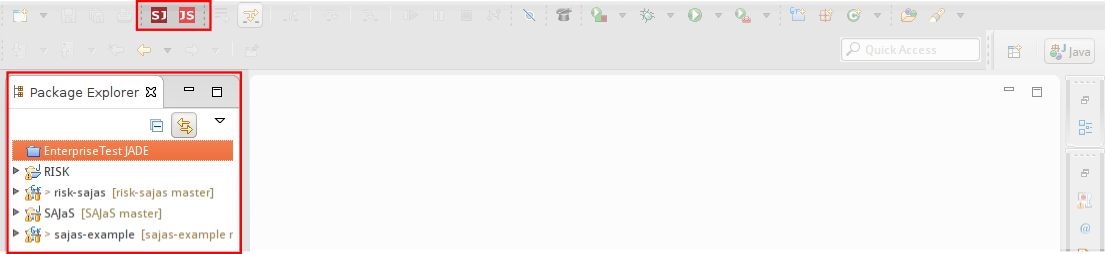
\includegraphics[width=\linewidth]{figures/cct_screenshot.png}
	\caption[Eclipse plugin screen capture]{Screen capture of Eclipse, showing the two plugin buttons and the Project Explorer view.}
	\label{fig:cct_screenshot}
\end{figure}

To run the plugin, a project should be selected from the Project Explorer and the button corresponding to the appropriate task should be pressed. The button 
\includegraphics[scale=1.0]{figures/sj.pdf} converts a SAJaS application into a JADE application and triggers the following actions:

\begin{samepage}
\begin{enumerate}
  \item Clone the selected project;
  \item Change all references to SAJaS classes in class imports;
  \item Inject \texttt{jade.jar} in the new project and add it to the build path;
  \item Fix hierarchy: classes that extended \texttt{RepastAgent} must now extend \texttt{Agent}
\end{enumerate}
\end{samepage}

The button 
\includegraphics[scale=1.0]{figures/js.pdf} converts a JADE application into a SAJaS application and triggers the following actions:

\begin{samepage}
\begin{enumerate}
  \item Create a Repast Project using a pre-made skeleton
  \item Copy the source code from the original project
  \item Change all references to JADE classes in class imports;
  \item Fix hierarchy: classes that extended \texttt{Agent} must now extend \texttt{RepastAgent}
\end{enumerate}
\end{samepage}

To perform the mapping of the class imports between the frameworks, dictionary file exists in the plugin's source. it allows for quick upgrades to the tool in the future. The dictionary also contains information regarding superclasses, i.e. those classes whose hierarchy needs to be fixed, as is the case of \texttt{RepastAgent} and \texttt{Agent}.